\chapter{Umsetzung der Webseite}
Die Digitalisierung hat enorme Auswirkungen auf Bildung und Lehre, und Hochschulen bilden da keine Ausnahme. Die DHBW Karlsruhe setzt sich, wie viele andere Bildungseinrichtungen auch, für die Nutzung digitaler Technologien ein, um das Lernen und die Bewältigung des Hochschullebens zu erleichtern. In diesem Zusammenhang entstand die Idee einer modernen Webseite, die speziell auf die Bedürfnisse der Studierenden der DHBW Karlsruhe zugeschnitten ist. Diese moderne Webseite soll die wichtigsten Informationen, die Studierende benötigen, auf effiziente und benutzerfreundliche Weise zusammenfassen.\\
\section{Ziel der Webseite}
Das Hauptziel der App besteht darin, den Informationsfluss zu optimieren und den Zugriff auf relevante Daten zu erleichtern. Ob Mensa-Speiseplan, aktuelle Vorlesung, Wochenplan oder eine Ansammlung von Links. Die Webseite sollte all diese Informationen an einem  zentralen Ort bereitstellen. Darüber hinaus möchten wir eine intuitive und ansprechende Benutzererfahrung bieten, die den Benutzern den Zugriff und die Navigation erleichtert.\\

\subsection{Wissenschaftliche Erkenntnisse} 
Zu den drei Hauptinformationen, die den Nutzern der DHBW Karlsruhe am wichtigsten sind, gehören Speisepläne, Stundenpläne und eine Sammlung nützlicher Links.\\
Der Kantinenplanung kommt eine große Bedeutung zu, da sie es Studierenden der DHBW Karlsruhe ermöglicht über den Tagesplan Bescheid zu wissen.\\
Auch Stundenpläne spielen eine wichtige Rolle, da sie den Studierenden helfen, ihre Kurse und Vorlesungen zu überschauen  und einen Überblick über ihre wöchentlichen Aktivitäten zu erhalten.\\ 
Darüber hinaus ist die Sammlung nützlicher Links eine wertvolle Ressource. Über diese Links erhalten Studierende einen einfachen Zugriff auf wichtige Online-Ressourcen und -Dienste, die sie regelmäßig nutzen. Dies ermöglicht einen schnellen Zugriff auf Informationen und unterstützende Materialien im Zusammenhang mit Ihren Lernbedürfnissen.\\ 
Insgesamt sind Mensapläne, Stundenpläne und eine Sammlung weiterführender Links die drei Hauptinformationen, die wir auf Basis unserer Erfahrung  für Studierende der DHBW Karlsruhe als am wichtigsten erachten. Durch die Optimierung dieser Informationen können Benutzer ihre täglichen Mahlzeiten einsehen, Unterrichtspläne effektiv überblicken und auf wichtige Online-Ressourcen zugreifen, um ihre Lernanforderungen zu erfüllen.\\
Die effektivsten Informationsquellen sind diejenigen, die den Benutzern einen schnellen und einfachen Zugriff auf die benötigten Informationen ermöglichen. In diesem Zusammenhang sind moderne  Webseiten , die auch für mobile Geräte optimiert ist, eine ideale Lösung, da sie die Möglichkeit bieten, alle notwendigen Informationen an einem Ort zu sammeln und sie den Benutzern jederzeit und überall zur Verfügung zu stellen.\\
Das Hauptproblem des Informationsangebots der DHBW Karlsruhe besteht in der Fragmentierung  und dem erschwerten Zugriff auf spezifische Informationen, da diese auf verschiedenen Plattformen verbreitet sind. Unser Vorschlag zur Lösung dieser Probleme ist die Entwicklung mobiler Webseiten. Diese Anwendung verbessert das Benutzererlebnis, indem sie die benötigten Informationen zentralisiert und es Benutzern ermöglicht, die benötigten Informationen schnell und einfach zu finden und zu verwenden.\\ 

\newpage
\section{Grundkonzept der Webseite}
Als mobile Informationsplattform konzipiert, zielt die Webseite darauf ab, die Informationsbeschaffung für Studierende der DHBW Karlsruhe zu optimieren und zu zentralisieren. Durch die Bündelung einer Vielzahl zusammengehöriger Dienste und Informationen und deren Darstellung auf einer intuitiven Benutzeroberfläche wollen wir den Informationsfluss optimieren und gleichzeitig einen hohen Komfort gewährleisten.
\subsection{Benutzeroberfläche}
Das Design der Benutzeroberfläche folgt den Designprinzipien Usability und User Experience (UX)  mit dem Ziel,  intuitive und benutzerfreundliche Anwendungen zu entwickeln\cite{hartmann2017usability}. Diese Prinzipien sind  für die Erstellung effizienter und effektiver Anwendungen, die die Benutzerzufriedenheit erhöhen, von wesentlicher Bedeutung\cite{14all}. Es orientiert sich an zeitgenössischen Designstandards und ist klar und minimalistisch gestaltet,da es dazu beiträgt, dass die Benutzeroberfläche übersichtlich und selbsterklärend bleibt\cite{massiveart}
Die wichtigsten Informationen und Dienste wie Speisepläne, Fahrpläne und Links sind direkt über die Startseite der Webseite zugänglich und werden mit sofort erkennbarer Ikonographie angezeigt..Dies erleichtert Benutzern die Navigation auf Ihrer Website und das Auffinden der benötigten Informationen. Durch die  Verwendung von Ikonografie zur Darstellung dieser Dienste sind diese sofort erkennbar und lassen sich in die Anwendung einfacher verwenden\cite{99designs}. 



\subsection{Navigation und Struktur}
Die Anwendung verwendet ein Seitenmenü zur Navigation. Dieses Menü enthält Symbole, die die Hauptbereiche der Anwendung darstellen, wie z. B. den Speiseplan, den Stundenplan und verschiedene Links.Durch Auswahl eines dieser Symbole gelangt der Benutzer direkt zu den entsprechenden Informationen. Diese Navigationsverwendung sorgt für eine uneingeschränkte  Anzahl von Menüpunkten, die sortierung der Menüpunkte nach Wichtigkeit un der Inhalt der Webseite beginnt direkt am oberen Rand und hat keine Einschränkung\cite{eology2023}.
Darüber hinaus ist die Struktur der Webseite logisch und hierarchisch aufgebaut, mit Seiten, die weitere Details oder spezifische Informationen bieten. Benutzer können zwischen diesen Seiten navigieren, indem sie wischen oder die entsprechenden Optionen in den Menüs auswählen.

\subsection{Funktion und Komponenten}
Die Webseite enthält verschiedene Funktionen und Komponenten, die darauf abzielen, Informationen effektiv anzuzeigen und gleichzeitig ein hohes Maß an Benutzerfreundlichkeit zu gewährleisten. 

Zu den Hauptmerkmalen gehören: 
\begin{itemize}
	\item Speiseplan: Diese Funktion zeigt das Tagesmenü an. Benutzer können sich auch zukünftige Menüs anzeigen lassen.
	\item Stundenplan: Eine Funktion, die den Stundenplan anzeigen lässt.
	\item Links: Diese Funktion bietet eine Sammlung verwandter Links, die Benutzern den einfachen Zugriff auf wichtige Online-Ressourcen und -Dienste ermöglichen.
\end{itemize}
\newpage
\section{Website-Komponenten}
In diesem Kapitel werden die einzelnen Funktionen und Komponenten erläutert-
\subsection{Home}
\subsubsection{Konzept}
Die Homepage ist als zentrale Informations- und Navigationsplattform konzipiert.Diese bietet einen  Überblick über die wichtigsten Informationen und Funktionen und dient gleichzeitig als Ausgangspunkt für die Navigation zu spezifischeren Seiten und Funktionen.  
Die Homepage ist in drei Hauptbereiche unterteilt.
\begin{itemize}
	\item Header:Die Kopfzeile enthält das Logo der Webseite sowie ein die Copyright Bezeichnung auf der rechten Seite. 
	\item Navigation: Die Navigation ist  in vertikaler Form am rechten Rand der Webseite konzipiert. Die enthält die Menüitems mit Symbolen, die den Hauptfunktionen der Webseite entsprechen. Durch Klicken auf diese Symbole gelangt der Benutzer direkt zur entsprechenden Seite.
	\item  Hauptbereich: Im Hauptbereich werden die Informationen angezeigt, die aktuell am relevantesten sind. Dazu gehören <die Angabe der jetzigen Vorlesung, der Mensaplan für den aktuellen Tag und eine Information für die aktuele Zeit.
\end{itemize} 
In dieser Abbildung ist die Visualisierung der Homepage dargestellt.\newpage
\begin{figure}[htbp]
	\centering
	\fbox{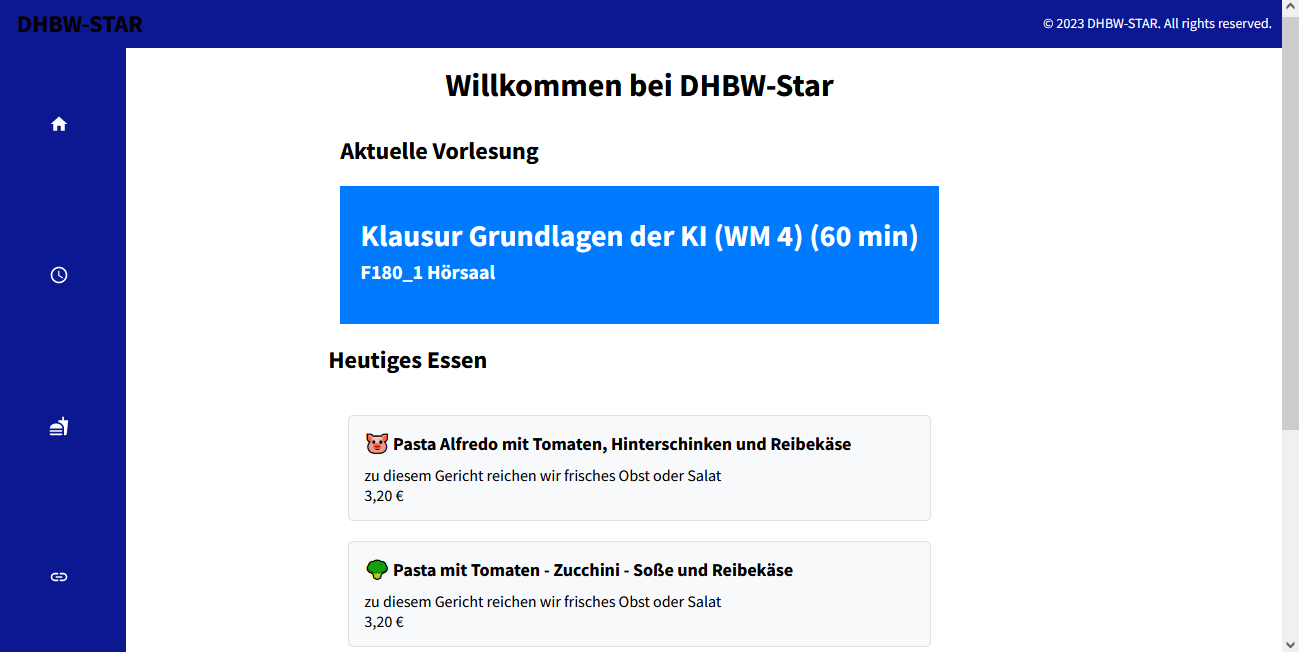
\includegraphics[height=0.3\textheight]{images/homepage}}
	\caption{Homepage}
\end{figure}
\subsubsection{Implementierung}
In diesem Codeblock befindet sich die Homepage-Komponente:\\
\begin{lstlisting}[language=JavaScript,
	frame=single,           % Ein Rahmen um den Code
	framexleftmargin=15pt,  % Rahmen link von den Zahlen
	style=algoBericht,
	label={Homepage-Komponente},
	captionpos=b ,          % Caption unter den Code setzen
	caption={Homepage-Komponente}]
import React, { useState, useEffect } from 'react';
import './home.css';
import SchedulerNow from '../Scheduler/ScheduleNow';
import FoodNow from '../Food/FoodNow';

function Homepage() {
    const [time, setTime] = useState(new Date());
    const [currentEvent, setCurrentEvent] = useState(null);
    useEffect(() => {
    	const interval = setInterval(() => {
          setTime(new Date());}, 1000);
        return () => clearInterval(interval);
     }, []);
    const days = ['Sonntag', 'Montag', 'Dienstag', 
    'Mittwoch', 'Donnerstag', 'Freitag', 'Samstag'];
    const today = days[time.getDay()];
    const date = time.toLocaleDateString();
    return (
    <div className="homepage">
    <div className="header">
    <h1>Willkommen bei DHBW-Star</h1>
    </div>
    <div className="current-lecture">
    <h2>Aktuelle Vorlesung</h2>
    <SchedulerNow setCurrentEvent={setCurrentEvent} />
    </div>
    <div className="todays-food">
    <h2>Heutiges Essen</h2>
    <FoodNow />
    </div>
    <div className="date-time">
    <h2>{today}, den {date}</h2>
    <h2>{time.toLocaleTimeString()}</h2>
    </div>
    </div>
    );
}
export default Homepage;
	
\end{lstlisting}

Die Homepage-Implementierung der DHBW Star-Webseite basiert auf der Nutzung grundlegender und erweiterter Funktionen der React-Bibliothek zur Erstellung der Benutzeroberfläche. Dieser Code verwendet React-Funktionen und Hooks, um eine dynamische und reaktionsfähige Benutzeroberfläche zu erstellen.\\ 
Die Hauptkomponente \emph{Homepage} wird als funktionale Komponente definiert.Funktionale Komponenten sind in modernen React-Anwendungen weit verbreitet, da sie einfacher zu lesen und zu testen sind und React-Hooks verwenden können.\\
Der Komponentenstatus wird über den \emph{useState}-Hook verwaltet. Dieser Hook ermöglicht es Komponenten, ihren eigenen Status beizubehalten und zu aktualisieren. In diesem Fall werden zwei Zustandsvariablen definiert: \emph{time} und \emph{currentEvent}.\\
Zur Darstellung der aktuellen Uhrzeit wird eine Zeitvariable verwendet, die jede Sekunde aktualisiert wird. Dies wird durch die Verwendung des \emph{useEffect}-Hooks erreicht. Dieser Hook führt eine Funktion aus, sobald die Komponente gerendert wird und wann immer sich der Status der Komponente ändert. Diese Funktion legt das Intervall zwischen Aufrufen der \emph{setTime}-Funktion jede Sekunde fest und aktualisiert die Zeitvariable. Die Variable \emph{currentEvent} wird verwendet, um das aktuell auftretende Vorlesung darzustellen. Dies wird durch Einbinden der \emph{SchedulerNow}-Komponente  und Übergeben der \emph{setCurrentEvent}-Funktion aktualisiert.\\ 
Die Homepage-Implementierung ist auf eine klare und einheitliche Struktur ausgelegt, sodass Nutzer auf einen Blick die wichtigsten Informationen wie aktuelle Uhrzeit, aktuelle Vorlesung, heutige Mahlzeit erkennen können. Darüber hinaus erleichtert diese Struktur die Erweiterung und Änderung der Homepage, wenn Sie in Zukunft weitere Funktionen oder Informationen hinzufügen müssen. React und seine Hooks ermöglichen eine effiziente Statusverwaltung und eine reaktionsfähige Benutzeroberfläche, die  automatisch aktualisiert wird, wenn sich der Status ändert.
\subsubsection{Programmablaufplan Homepage}
In dieser Abbildung wird der Ablauf der Komponenten visualisiert:
\begin{figure}[htbp]
	\centering
	\fbox{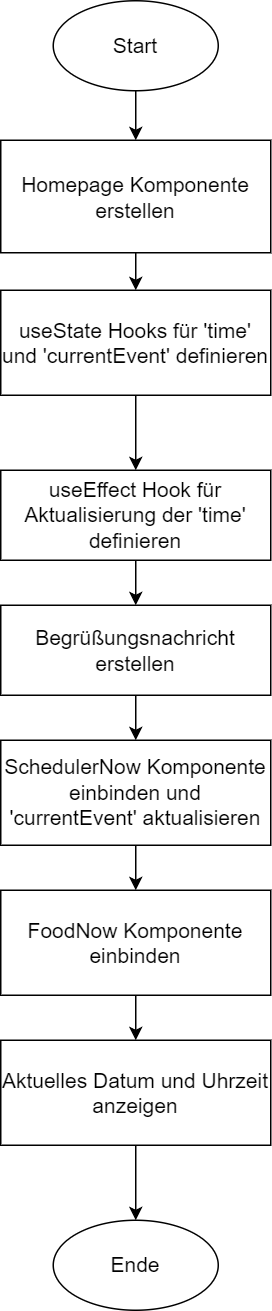
\includegraphics[height=0.5\textheight]{images/PAPHomepage}}
	\caption{PAP Homepage}
\end{figure}

\subsection{Food}
\subsubsection{Konzept}
Die Food-Komponente der DHBW Star-Webseite ist ein wichtiger Teil der Anwendung,die Speisepläne anzeigt.
Die Daten werden von einer Mensa-APi abgerufen die in einem Docker-Container erstellt wird. Dieser Vorgang wird in dem Kapitel Docker näher beschrieben.
Der Default-Speiseplan ist immer der aktuelle Tag, zu dem werden für die nächsten zehn Tage die Speisepläne angezeigt. Außer an Wochenenden, da ist die Mensa geschlossen.
In diesem Programmablaufplan ist die Food-Komponente visuell erklärt.\\
\begin{figure}[htbp]
	\centering
	\fbox{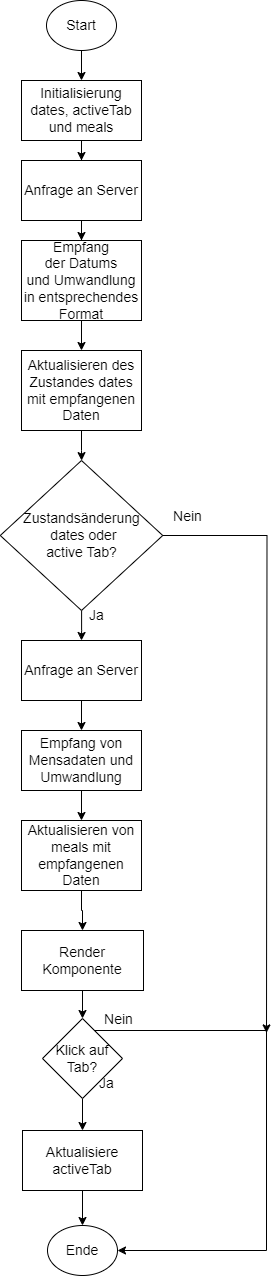
\includegraphics[height=0.65\textheight]{images/PAPFood}}
	\caption{PAP Food}
\end{figure}
 \newpage
 Zudem ist in der nächsten Abbildung die Webseite der Food-Komponente abgebildet.
 \begin{figure}[htbp]
 	\centering
 	\fbox{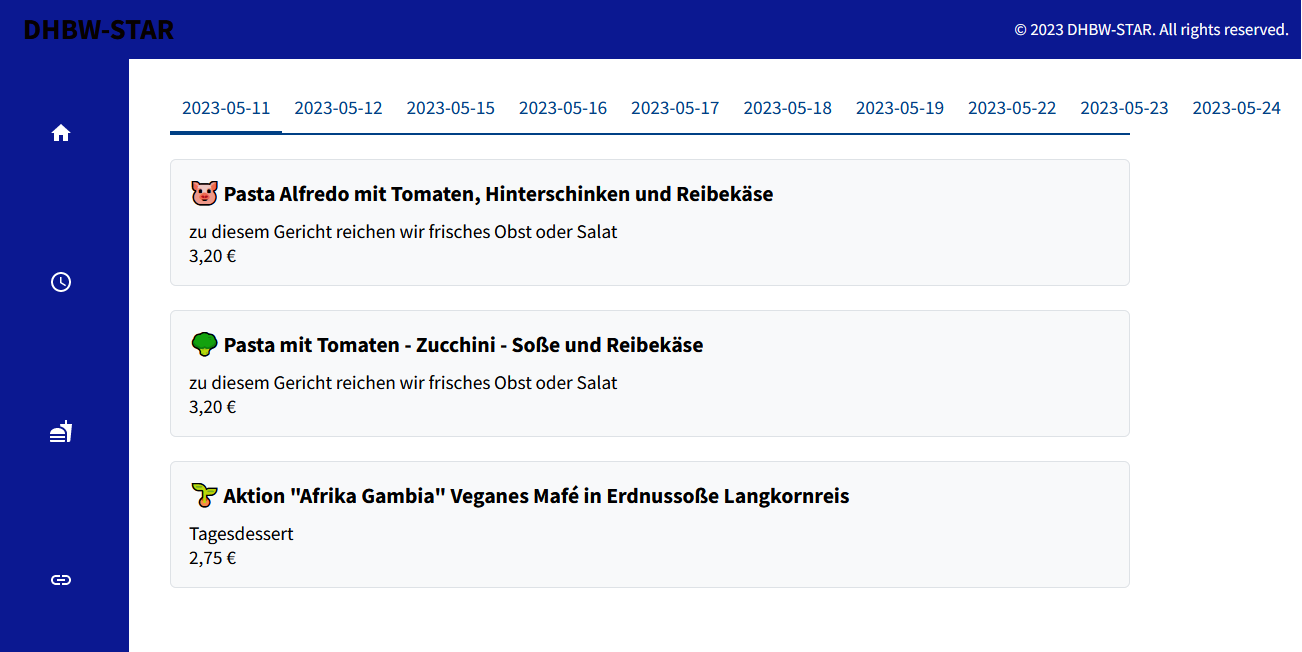
\includegraphics[height=0.3\textheight]{images/Food}}
 	\caption{Food Website}
 \end{figure}
\subsubsection{Implementierung}
Die Implementierung der Foodkomponente der DHBW Star-Webseite basiert auf der Verwendung grundlegender und erweiterter Funktionen der React- und \emph{Axios}-Bibliotheken zur Verarbeitung von HTTP-Anfragen.
Die \emph{Food}-Komponente wird als funktionelle Komponenten definiert und nutzt React-Hooks, um den internen Zustand und Nebenwirkungen zu verwalten. Mit dem Hook \emph{useState} werden drei Statusvariablen definiert: \emph{dates}, \emph{activeTab} und \emph{meals}. \emph{Dates} speichert  Daten, an denen Mahlzeiten verfügbar sind, \emph{activeTab} speichert den Index des aktuell ausgewählten Datums und \emph{Meals} speichert Mahlzeitinformationen für das aktuell ausgewählte Datum. Der \emph{useEffect}-Hook wird zweimal verwendet. Einmal, um das Datum abzurufen, an dem die Komponente zum ersten Mal gerendert wird, und einmal, um die Informationen zur Essenszeit abzurufen, wenn sich das aktive Datum ändert. Die Funktionen \emph{fetchDates} und \emph{fetchMeals} verwenden die \emph{Axios}-Bibliothek, um eine HTTP-GET-Anfrage an den Server zu senden, um Daten abzurufen. 
Informationen zu Mahlzeiten werden angezeigt, indem das Array \emph{Meals} durchlaufen und  für jede Mahlzeit ein JSX-Element generiert wird. Es verwendet die Funktion \emph{getEmoji}, um passende Emojis basierend auf Essensklassifikatoren zu generieren.\\
Dies ist der dazugehörige Code:
\newpage
\begin{lstlisting}[language=JavaScript,
	frame=single,           % Ein Rahmen um den Code
	framexleftmargin=15pt,  % Rahmen link von den Zahlen
	style=algoBericht,
	label={Food-Komponente},
	captionpos=b ,          % Caption unter den Code setzen
	caption={Food-Komponente}]
import React, { useState, useEffect } from "react";
import axios from "axios";
import "./Food.css";

const getEmoji = (classifier,name) => {
     switch (classifier) {
     	case "S":
        return "\emoji{pig face}";
        case "SAT":
        return "\emoji{pig face}";
        case "R":
        return "\emoji{cow face}";
        case "RAT":
        return "\emoji{cow face}";
        case "MSC":
        return "\emoji{fish}";
        case "VEG":
        return "\emoji{broccoli}";
        case "VG":
        return "\emoji{seedling}";
        case "N":
        return "\\emoji{person gesturing NO}";
        default:
        return "\emoji{forkandknifewithplate️}";
    }
};
const Food = () => {
    const [dates, setDates] = useState([]);
    const [activeTab, setActiveTab] = useState(0);
    const [meals, setMeals] = useState([]);
    
    useEffect(() => {
    fetchDates();
     }, []);
	
    useEffect(() => {
        if (dates.length > 0) {
        fetchMeals(dates[activeTab]);
    }
    }, [dates, activeTab]);
	
    const fetchDates = async () => {
       try {
         const response = await axios.get(process.env.
         REACT_APP_MENSA_ADDRESS+"/plans");
         const dateList = response.data.data.map((date) =>
         `{date.date.year}-{(date.date.month + 1).toString()
         	.padStart(2, "0")}-{date.date.day.toString()
         	.padStart(2, "0")}`
          ).slice(0, 10);
          setDates(dateList);
         } catch (error) {
		  console.error("Error fetching dates:", error);
			}
		};
	
      const fetchMeals = async (date) => {
         try {
            const response = await axios.get(
            process.env.REACT_APP_MENSA_ADDRESS+
            `/plans/{date}?canteens=erzberger`
			);
            let mealData = response.data.data[0].lines
            .slice(0, 3)
            .map((line) => ({
                main: line.meals[0],
                description: line.meals[1]?.name,}));
            if (!mealData[0]['main']){
            	console.log("FEIERTAG")
            	mealData=[{
            	    main: {
            	        classifiers: 'Nein',
            	        name:"Feiertag/kein Essen",
            	        price:"0 Euro"
                    },
                    description: "An dem heutigen Tag ist 
                    die Mensa geschlossen."}]
                }
            setMeals(mealData);
        } catch (error) {
           console.error("Error fetching meals:", error);
	    }
    };
    
    return (
    <div className="mensa-plan">
    <div className="tabs">
    {dates.map((date, index) => (
        <button
        key={index}
        className={`tab {index === activeTab ? "active" : ""}`}
        onClick={() => setActiveTab(index)}
        >
        {date}
        </button>
        ))}
    </div>
    <div className="tab-content">
    {meals.map((mealObj, index) => {
            const meal = mealObj.main;
            if (meal?.empty) {
                return (
                <div key={index} className="no-meal">
                <h3>Feiertag/Kein Essen</h3>
                </div>
                );
            } else {
            return (
            <div key={index} className="meal">
            <h3>
            {getEmoji(meal.classifiers[0],meal.name)} {meal.name}
            </h3>
            <p>{mealObj.description}</p>
            <p>{meal.price}</p>
            </div>
            );}
        })}
    </div>
	</div>
	);
};

export default Food;

\end{lstlisting}

Die Implementierung der \emph{Food}-komponente wurde so konzipiert, dass Datenerfassung und -präsentation sauber getrennt werden. Mit React-Hooks ist es möglich den Komponentenstatus effizient zu verwalten und die Benutzeroberfläche automatisch zu aktualisieren, wenn sich der Status ändert. Die \emph{Axios}-Bibliothek macht die Bearbeitung von HTTP-Anfragen einfach und zuverlässig. Diese Struktur ermöglicht auch eine einfache Anpassung und Erweiterung der Komponente, wenn in Zukunft zusätzliche Funktionen oder Änderungen erforderlich sind.

\subsubsection{FoodNow}
Die \emph{FoodNow}-Komponente der DHBW-Star-Webseite wurde entwickelt, um Nutzern aktuelle Informationen zur Essensverfügbarkeit in der Mensa zur Verfügung zu stellen. Es wurde mithilfe der React- und Axios-Bibliotheken zur Verwaltung von HTTP-Anfragen implementiert. 
Diese Komponente besteht aus Funktionskomponenten, die mithilfe der \emph{useState}- und \emph{useEffect}-Hooks von React den Status verwalten und Nebenwirkungen behandeln. Es werden zwei Zustandsvariablen definiert. Das eine ist \emph{meals}, das die aktuell verfügbaren Mahlzeiten speichert, und das andere ist \emph{mensaStatus}, das den aktuellen Status des Restaurants speichert (geöffnet oder kurz vor der Eröffnung). 
Der \emph{useEffect}-Hook wird verwendet, um die \emph{fetchMeals}-Funktion auszulösen, sobald die Komponente in der Benutzeroberfläche gerendert wird. Diese Funktion ruft zunächst die Funktion \emph{isMensaOpen} auf, um zu sehen, ob die Mensa geöffnet ist oder kurz vor der Eröffnung steht. Diese Funktion überprüft das aktuelle Datum und die aktuelle Uhrzeit und vergleicht sie mit den  Öffnungs- und Schließzeiten des angegebenen Restaurants. 
Wenn die Mensa geöffnet ist oder kurz vor der Eröffnung steht, wird eine HTTP-GET-Anfrage an den Mensa-Server gesendet, um die verfügbaren Mahlzeiten für den  Tag abzurufen. Erhaltene Mahlzeiten werden  im Status \emph{meals} gespeichert und der Status der Mensa wird in \emph{mensaStatus} gespeichert. 
Die Rendermethode der Komponente prüft, ob die Cafeteria geöffnet ist oder kurz vor der Eröffnung steht und stellt die verfügbaren Mahlzeiten entsprechend dar oder zeigt eine Meldung an, dass die Cafeteria geschlossen ist oder kurz vor der Eröffnung steht. Die Implementierung der \emph{FoodNow}-Komponente auf diese Weise ermöglicht eine effiziente Handhabung von Statusänderungen und Nebenwirkungen und hält die Benutzeroberfläche auf dem neuesten Stand. Die Axios-Bibliothek erleichtert Komponenten das Senden und Empfangen von HTTP-Anfragen. Diese Implementierung trägt dazu bei, dass der Code sauber und  organisiert bleibt, wodurch er einfacher zu lesen und zu warten ist.
In diesem Codeblock befindet sich der dazugehörige Code:
\begin{lstlisting}[language=JavaScript,
	frame=single,           % Ein Rahmen um den Code
	framexleftmargin=15pt,  % Rahmen link von den Zahlen
	style=algoBericht,
	label={FoodNow-Komponente},
	captionpos=b ,          % Caption unter den Code setzen
	caption={FoodNow-Komponente}]
import React, { useState, useEffect } from "react";
import axios from "axios";
import "./Food.css";
const getEmoji = (classifier, name) => {
  switch (classifier) {
  	case "S":
  	return "🐷";
  	case "SAT":
  	return "🐷";
  	case "R":
  	return "🐮";
  	case "RAT":
  	return "🐮";
  	case "MSC":
  	return "🐟";
  	case "VEG":
  	return "🥦";
  	case "VG":
  	return "🌱";
  	case "N":
  	return "🙅";
  	default:
  	return "🍽️";
 }};

const FoodNow = () => {
   const [meals, setMeals] = useState([]);
   const [mensaStatus, setMensaStatus] = 
   useState({ isOpen: false, isBeforeOpening: false });
   
   useEffect(() => {
   fetchMeals();}, []);

   const isMensaOpen = () => {
    const now = new Date();
    const day = now.getDay();
    const time = now.getHours() * 60 + now.getMinutes();
    const openingTime = 11 * 60 + 15;
    const closingTime = 13 * 60 + 30;
 
    const beforeOpening = time < openingTime;
    return {
    	isOpen: day >= 1 && day <= 5 && time >= openingTime 
    	&& time <= closingTime,
    	isBeforeOpening: beforeOpening,};
    };
   const fetchMeals = async () => {
   	 try {
   	  const mensaStatus = isMensaOpen();
   	  if (mensaStatus.isOpen || mensaStatus.isBeforeOpening) {
   	    const today = new Date().toISOString().slice(0, 10);
   	    const response = await axios.get(
   	    process.env.REACT_APP_MENSA_ADDRESS+
   	    `/plans/${today}?canteens=erzberger`);
   	    let mealData = response.data.data[0].lines.slice(0, 3)
		.map((line) => ({
		  main: line.meals[0],
		  description: line.meals[1]?.name,}));
		 if (!mealData[0]["main"]) {
		 	console.log("FEIERTAG");
		 	mealData = [{
		 		main: {
		 		  classifiers: "Nein",
		 		  name: "Feiertag/kein Essen",
		 		  price: "0",},
	 		    description: "An dem heutigen Tag ist 
	 		    die Mensa geschlossen.",},];
 		    }
 	     setMeals(mealData);
 	     setMensaStatus(mensaStatus);
      } else {
         setMensaStatus({ isOpen: false, isBeforeOpening: false });}
	} catch (error) {
	    console.error("Error fetching meals:", error);}
   };

   return (
   <div className="mensa-plan">
   <div className="tab-content">
   {mensaStatus.isOpen || mensaStatus.isBeforeOpening ? (
   	 meals.length > 0 ? (
   	 meals.map((mealObj, index) => {
   	   const meal = mealObj.main;
   	   return (
   	   <div key={index} className="meal">
   	   <h3>
   	   {getEmoji(meal.classifiers[0], meal.name)}{meal.name}
   	   </h3>
   	   <p>{mealObj.description}</p>
   	   <p>{meal.price}</p>
   	   </div>
	);})
	) : (
	  <div className="no-meal">
	  <h3>Keine Informationen fuer 
	  heute verfuegbar</h3>
	  </div>)
	) : (
	  <div className="no-meal">
	  <h3>Die Mensa ist geschlossen</h3>
	  </div>)}
   {mensaStatus.isBeforeOpening && (
   	<div className="before-opening">
   	<h3>Die Mensa ist noch geschlossen. 
   	Sie oeffnet um 11:15 Uhr.</h3>
   	</div>)}
	</div>
	</div>
	);
};
export default FoodNow;
	
\end{lstlisting}
\newpage
\subsection{Scheduler}
\subsubsection{Konzept}
Die \emph{Scheduler}-Komponente wurde entwickelt, um Nutzern einen Überblick über geplante Vorlesungen in der DHBW-Star-Webseite zu geben. Es wurde mithilfe der React-Bibliothek, der Axios-Bibliothek zum Verwalten der HTTP-Anfragen und der FullCalendar-Bibliothek zum Rendern der Ereignisse im Kalender implementiert.\\
Die Webseite der \emph{Scheduler}-Komponente ist in dieser Abbildung dargestellt.\\
\begin{figure}[htbp]
	\centering
	\fbox{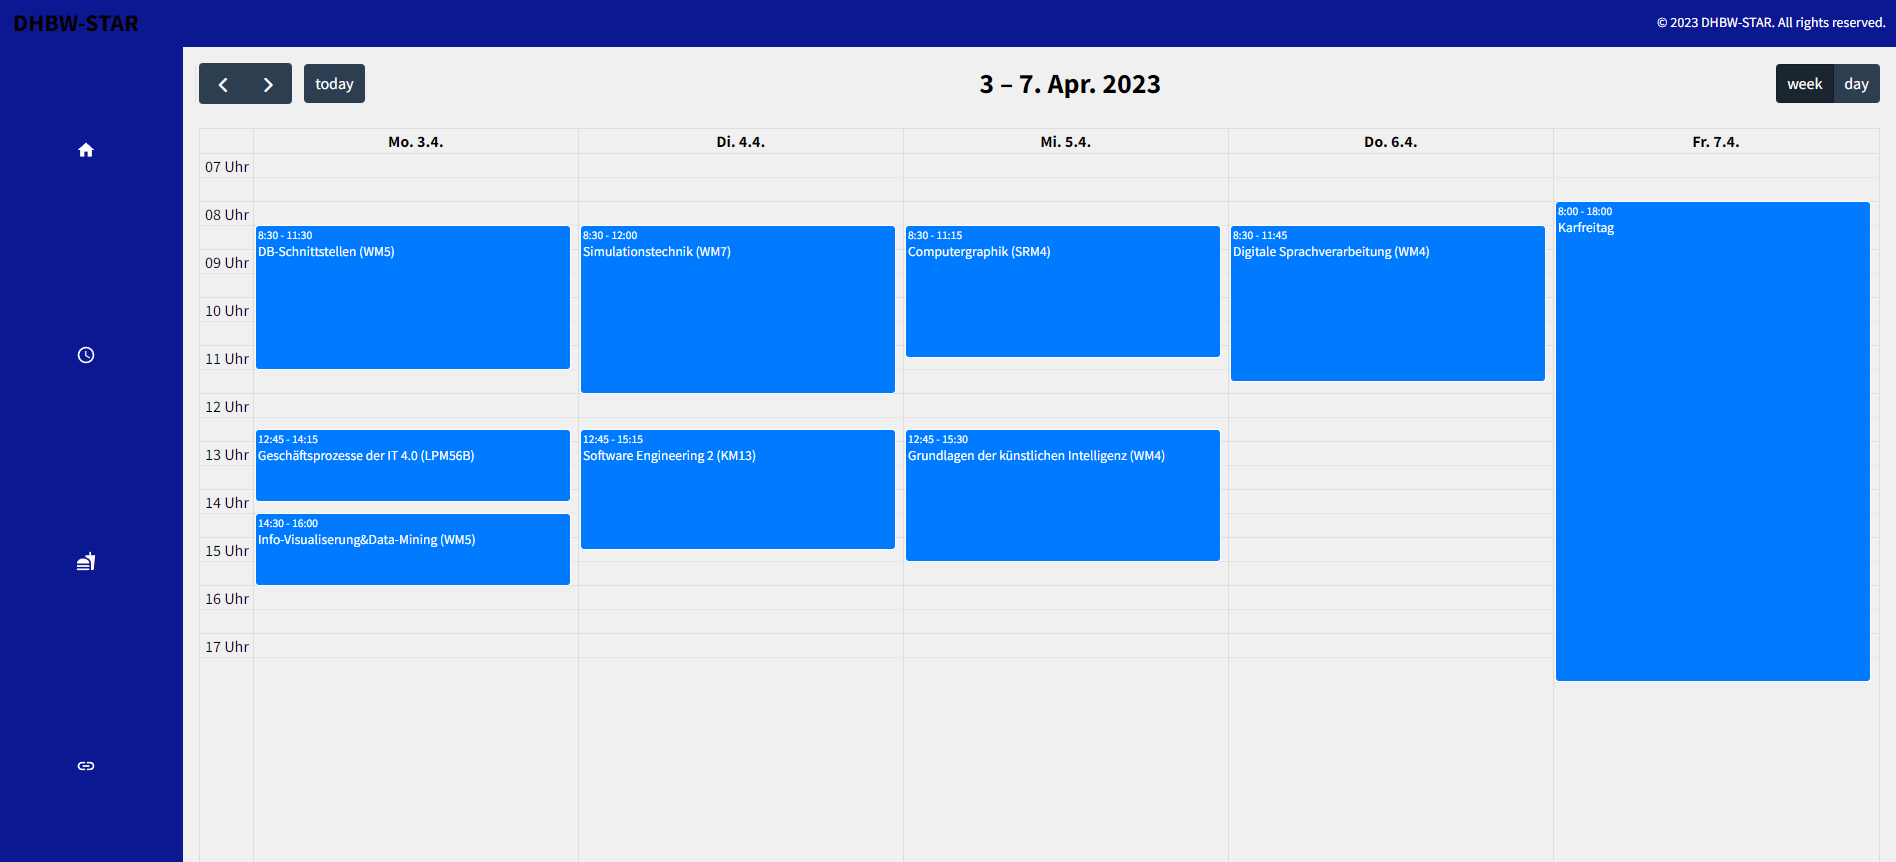
\includegraphics[height=0.35\textheight]{images/Scheduler}}
	\caption{Scheduler}
\end{figure}
\newpage
Die Grundschritte der Implementierung werden in diesem Programmablaufplans visualisiert um die Grundfunktion verständlicher zu machen.
\begin{figure}[htbp]
	\centering
	\fbox{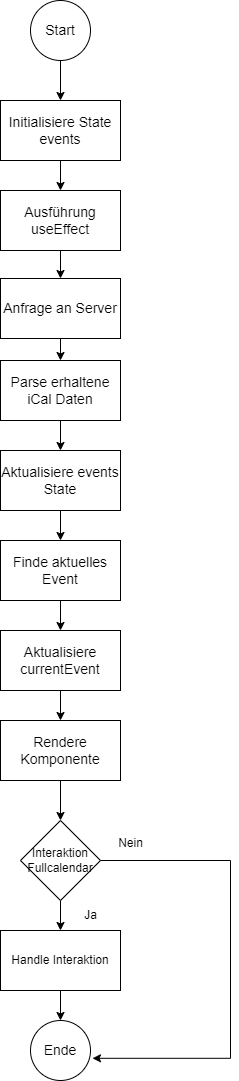
\includegraphics[height=0.65\textheight]{images/PAPScheduler}}
	\caption{PAP Scheduler}
\end{figure}
\newpage
\subsubsection{Implementierung}
Das ist der Code für die \emph{Scheduler}-Komponente:
\begin{lstlisting}[language=JavaScript,
	frame=single,           % Ein Rahmen um den Code
	framexleftmargin=15pt,  % Rahmen link von den Zahlen
	style=algoBericht,
	label={Scheduler-Komponente},
	captionpos=b ,          % Caption unter den Code setzen
	caption={Scheduler-Komponente}]
import React, { useState, useEffect } from 'react';
import axios from 'axios';
import FullCalendar from '@fullcalendar/react';
import dayGridPlugin from '@fullcalendar/daygrid';
import timeGridPlugin from '@fullcalendar/timegrid';
import interactionPlugin from '@fullcalendar/interaction';
import './Scheduler.css';
import ICAL from 'ical.js';
import '@fullcalendar/core/locales-all';
import { isWithinInterval } from 'date-fns';

const Scheduler = ({ setCurrentEvent }) => {
    const [events, setEvents] = useState([]);
    
    useEffect(() => {
         const fetchData = async () => {
            try {
               const response = await 
               axios.get(
               process.env.REACT_APP_PROXY_ADDRESS+'/schedule');
               const data = response.data;
               const parsedEvents = parseEvents(data);
               setEvents(parsedEvents);
               const currentEvent = getCurrentEvent(parsedEvents);
               setCurrentEvent(currentEvent);
           } catch (error) {
               console.error(
               'Error fetching schedule data:', error);
           }};
       fetchData();
   }, [setCurrentEvent]);

       const getCurrentEvent = (events) => {
       	  const now = new Date();
       	  const currentEvent = events.find(
       	  (event) =>
       	  isWithinInterval(now, 
       	  { start: event.start, end: event.end }) &&
       	  now.getTime() <= event.end.getTime()
       	  );
       	  return currentEvent;
       };
      
      const parseEvents = (icalData) => {
        const jcalData = ICAL.parse(icalData);
        const comp = new ICAL.Component(jcalData);
        const events = comp.getAllSubcomponents('vevent');
        const now = new Date();
        const startDate = ICAL.Time.fromJSDate(
        new Date(now.getFullYear() - 1, 
        now.getMonth(), now.getDate()));
        const endDate = ICAL.Time.fromJSDate(
        new Date(now.getFullYear() + 1, 
        now.getMonth(), now.getDate()));
        const parsedEvents = [];
        events.forEach(eventComponent => {
           const event = new ICAL.Event(eventComponent);
           const start = event.startDate;
           const end = event.endDate;
           
           if (event.isRecurring()) {
           	const iterator = event.iterator();
           	let next;
            while ((next = iterator.next())) {
                if (next.compare(startDate) < 0) {
                    continue;}
                if (next.compare(endDate) > 0) {
                	break;}
                const duration = end.subtractDate(start);
                const eventStart = next;
                const eventEnd = eventStart.clone();
                eventEnd.addDuration(duration);
                    parsedEvents.push({
                       title: event.summary,
                       start: eventStart.toJSDate(),
                       end: eventEnd.toJSDate(),
                       location: event.location ? 
                       event.location.value : '',
                       description: event.description,});}
             } else {
               parsedEvents.push({
                title: event.summary ,
               	start: start.toJSDate(),
               	end: end.toJSDate(),
               	location: event.location,
               	description: event.description,
               });
           }
       });
        console.log(parsedEvents);
        return parsedEvents;
    };
    return (
    <div className="scheduler">
    <FullCalendar
    plugins={[dayGridPlugin, timeGridPlugin, interactionPlugin]}
    initialView="timeGridWeek"
    headerToolbar={{
    	left: 'prev,next today',
    	center: 'title',
    	right: 'timeGridWeek,timeGridDay',}}
    events={events}
    eventColor="#007bff" //// Blaue Akzente
    locale="de"
    allDaySlot={false} // Entfernt die Anzeige fuer "all day"-Events
    nowIndicator={true} 
    // Fuegt einen roten Zeitstrahl fuer die aktuelle Zeit hinzu
    weekends={false} // Versteckt Wochenenden
    slotMinTime="07:00:00" // Startzeit fuer Zeitslots
    slotMaxTime="18:00:00" // Endzeit fuer Zeitslots
    />
    </div>
    );
};
export default Scheduler;
\end{lstlisting}
Die \emph{Scheduler}-Komponente besteht aus Funktionskomponenten, die die React-Hooks \emph{useState} und \emph{useEffect} verwenden, um den Status zu verwalten und Nebenwirkungen zu behandeln. Der \emph{useState}-Hook wird verwendet, um den Status des im Kalender angezeigten Ereignisses zu speichern,  und der \emph{useEffect}-Hook wird verwendet, um die \emph{fetchData}-Funktion auszulösen, sobald die Komponente in der Benutzeroberfläche angezeigt wird.\\
Die \emph{fetchData}-Funktion sendet eine HTTP-GET-Anfrage an den Server,um \emph{ical}-Daten für geplante Ereignisse abzurufen. Diese Daten werden dann mithilfe der \emph{parseEvents}-Funktion in ein Format konvertiert, das von der \emph{FullCalendar}-Bibliothek verstanden wird. Diese Funktion verwendet die \emph{ICAL.js}-Bibliothek, um die \emph{ical}-Daten zu analysieren und in ein JavaScript-Objekt zu konvertieren. Es berücksichtigt auch wiederkehrende Ereignisse und generiert für jede Wiederholung innerhalb eines bestimmten Zeitraums ein eigenes Ereignis.\\
Die Funktion \emph{getCurrentEvent} wird verwendet, um das aktuelle Ereignis abzurufen, also das Ereignis, das gerade auftritt. Diese durchsucht die Liste der Ereignisse nach Ereignissen, deren Start- und Endzeit das aktuelle Datum enthalten. Dieses Ereignis wird zur Anzeige durch eine andere Komponente in der Anwendung an die übergeordnete Komponente zurückgegeben.\\
Schließlich gibt die \emph{Scheduler}-Komponente eine \emph{FullCalendar}-Komponente zurück, die mit  entsprechenden Eigenschaften konfiguriert ist, um die Ereignisse benutzerfreundlich anzuzeigen.Die Komponente nutzt mehrere Plugins von FullCalendar, um unterschiedliche Ansichten und Interaktionen zu ermöglichen.\\
Diese Art und Weise der Implementierung bietet eine effiziente und flexible Möglichkeit, geplante Ereignisse anzuzeigen. Es stellt sicher, dass die Daten immer auf dem neuesten Stand sind und ermöglicht Benutzern eine einfache und intuitive Übersicht ihrer Veranstaltungen. Die Verwendung etablierter Bibliotheken wie \emph{Axios}, \emph{FullCalendar} und \emph{ICAL.js} reduziert die Codekomplexität und erhöht die Zuverlässigkeit und Wartbarkeit.
\subsubsection{Proxy-Server}

Der Proxy-Server ist so konzipiert, dass er die Cross-Origin Resource Sharing (CORS)-Richtlinie umgeht, die von APIs auferlegt werden. Eine CORS-Richtlinie ist eine Sicherheitsmaßnahme, die von Browsern angewendet wird, um  unerwünschten Datenzugriff über verschiedene Domänen hinweg zu verhindern. In diesem Fall verbietet die CORS-Richtlinie der API \emph{'http://rapla.dhbw-karlsruhe.de/rapla?page=iCal\&user=vollmer\&file=tinf20b3'} den direkten Clientzugriff auf die Kalenderdaten. Um dieses Problem zu lösen, wurde ein Proxy-Server entwickelt, der als Vermittler zwischen Clients und API/Server fungiert. Dieses Bild veranschaulicht die Rolle des Proxy-Servers genauer.
\begin{figure}[htbp]
	\centering
	\fbox{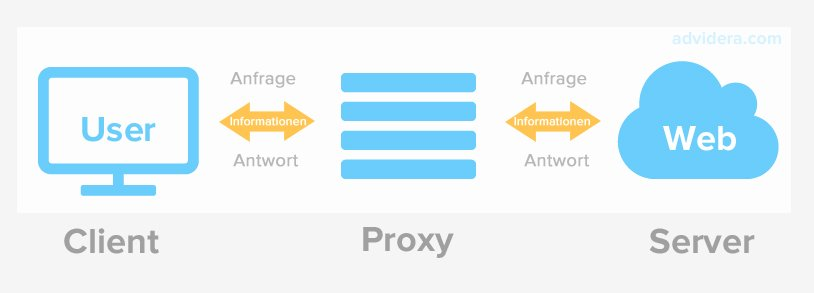
\includegraphics[height=0.25\textheight]{images/Proxyserver}}
	\caption{Proxy-Server}
\end{figure}

Der Proxy-Server wurde in \emph{Node.js} mithilfe des Express-Frameworks implementiert, das ein benutzerfreundliches Framework zum Erstellen von Webanwendungen und APIs bietet. Zudem wurde das CORS-Paket importiert, um \emph{Axios} zum Senden von HTTP-Anfragen an CORS-Funktionen und APIs bereitzustellen.\\
Ein Cache-Objekt wurde eingeführt, um  Antwortdaten für einen bestimmten Zeitraum (in diesem Fall 1 Stunde) zu speichern und unnötige Anfragen an die API zu vermeiden. Diese Cache-Implementierung trägt dazu bei, die API-Last zu reduzieren und die Anwendungsleistung zu verbessern, indem  die Anzahl der an die API gesendeten Anforderungen reduziert wird. Wenn die Anfrage innerhalb des Cache-Zeitraums wiederholt wird, werden die zwischengespeicherten Daten an den Client gesendet, ohne erneut auf die API zuzugreifen.\\
Die Proxy-Anwendung stellt einen einzelnen Endpunkt \emph{/schedule} bereit, um Kalenderdaten auf Anfrage asynchron abzurufen. Zunächst prüft es, ob sich die Daten im Cache befinden und innerhalb des Cache-Zeitraums noch  gültig sind. Falls vorhanden, werden die zwischengespeicherten Daten an den Client gesendet. Andernfalls wird eine Anfrage an die API gesendet, um die neuesten Kalenderdaten abzurufen.Antwortdaten werden zwischengespeichert und an den Client gesendet.\\
Der Proxy-Server läuft auf Port 3002 oder einem anderen Port, der durch die Umgebungsvariable \emph{PROXYPORT} angegeben wird. Der Proxy-Server ermöglicht es der Scheduler-Anwendung, CORS-Richtlinien zu umgehen und auf die Kalenderdaten der API zuzugreifen, um sie im Client darzustellen.\
Dies ist der zu entsprechende Code:
\begin{lstlisting}[language=JavaScript,
	frame=single,           % Ein Rahmen um den Code
	framexleftmargin=15pt,  % Rahmen link von den Zahlen
	style=algoBericht,
	label={Proxy-Server},
	captionpos=b ,          % Caption unter den Code setzen
	caption={Proxy-Server}]
const express = require('express');
const cors = require('cors');
const axios = require('axios');
const cach = {}
const cachDuration = 3600000; //1h
const kurs = 'tinf20b3'
const app = express();
app.use(cors());
app.get('/schedule', async (req, res) => {
  if (kurs in cach && cach['tinf20b3']
  .time > new Date().getTime())
  { console.log("Get cached Data");
  	res.send(cach['tinf20b3'].data);}
  else{
    try {
      const response = await axios.get(
      'http://rapla.dhbw-karlsruhe.de/rapla?
      page=iCal&user=vollmer&file=tinf20b3');
      cach[kurs] = {
      	time: new Date().getTime() + cachDuration,
      	data: response.data};
      console.log("save Data in cache:" + cach['tinf20b3'].time);
      res.send(response.data);} 
   catch (error) {res.status(500).send({ error: 
   	   'An error occurred while fetching the data.' });}}});
const PORT = process.env.PROXY_PORT || 3002;
app.listen(PORT, () => console.log(`Proxy 
server running on port ${PORT}`));

\end{lstlisting}
\subsubsection{SchedulerNow}
Die Komponente \emph{SchedulerNow} ist eine spezielle Komponente, die entwickelt wurde, um  aktuelle Ereignisse (z. B. laufende Vorlesungen) aus dem iCalendar-Format (iCal) zu extrahieren und anzuzeigen. Diese Komponente ist in React geschrieben und verwendet \emph{useState}- und \emph{useEffect}-Hooks, um den internen Status zu verwalten. Dieser Code entspricht der \emph{SchedulerNow}-Komponente:

\begin{lstlisting}[language=JavaScript,
	frame=single,           % Ein Rahmen um den Code
	framexleftmargin=15pt,  % Rahmen link von den Zahlen
	style=algoBericht,
	label={SchedulerNow-Komponente},
	captionpos=b ,          % Caption unter den Code setzen
	caption={SchedulerNow-Komponente}]
import React, { useState, useEffect } from 'react';
import axios from 'axios';
import ICAL from 'ical.js';
import { isWithinInterval } from 'date-fns';
import './SchedulerNow.css';

const SchedulerNow = () => {
   const [currentEvent, setCurrentEvent] = useState(null);
   useEffect(() => {
   	const fetchData = async () => {
   	  try {
   	    const response = await axios.get(process.env.
   	    REACT_APP_PROXY_ADDRESS+'/schedule');
   	    const data = response.data;
   	    const parsedEvents = parseEvents(data);
   	    const currentEvent = getCurrentEvent(parsedEvents);
   	    setCurrentEvent(currentEvent);
       } catch (error) {
        console.error('Error fetching schedule data:', error);}
    };
    fetchData();}, []);
    
    const getCurrentEvent = (events) => {
       const now = new Date();
       const currentEvent = events.find(
       (event) => isWithinInterval(now, 
       { start: event.start, end: event.end }));
       return currentEvent;};
   
   const parseEvents = (icalData) => {
     const jcalData = ICAL.parse(icalData);
     const comp = new ICAL.Component(jcalData);
     const events = comp.getAllSubcomponents('vevent');
     const now = new Date();
     const startDate = ICAL.Time.fromJSDate(new Date(
     now.getFullYear(), now.getMonth()-1, now.getDate()));
     const endDate = ICAL.Time.fromJSDate(new Date(
     now.getFullYear() + 1, now.getMonth(), now.getDate()));
     const parsedEvents = [];
     events.forEach(eventComponent => {
       const event = new ICAL.Event(eventComponent);
       const start = event.startDate;
       const end = event.endDate;
       if (event.isRecurring()) {
       	const iterator = event.iterator();
       	let next;
       	while ((next = iterator.next())) {
       	  if (next.compare(startDate) < 0) {
       	  	continue;}
          if (next.compare(endDate) > 0) {
          	break;}
         const duration = end.subtractDate(start);
         const eventStart = next;
         const eventEnd = eventStart.clone();
         eventEnd.addDuration(duration);
          parsedEvents.push({
            title: event.summary,
            start: eventStart.toJSDate(),
            end: eventEnd.toJSDate(),
            location: event.location ? event.location.value : '',
            description: event.description,});
        }
    } else {
     parsedEvents.push({
       title: event.summary ,
       start: start.toJSDate(),
       end: end.toJSDate(),
       location: event.location,
       description: event.description,});
   }});
  console.log('Parsed events:', parsedEvents);
  return parsedEvents;};

  const renderCurrentEvent = () => {
    console.log('Current event:', currentEvent);
    if (!currentEvent) {
    	return <div className="no-lecture">Keine Vorlesung</div>;}
    return (
    <div className="current-lecture">
    <div className="title">{currentEvent.title}</div>
    {currentEvent.location && (
      <div className="location">{currentEvent.location}</div>
	)}
    </div>);
   };
 return (
 <div className="scheduler-now">
 {renderCurrentEvent()}</div>);};

export default SchedulerNow;
\end{lstlisting}

Zunächst wird der Zustand \emph{currentEvent} initialisiert, der das aktuelle Ereignis darstellt. Dieser Status wird später aktualisiert, wenn Daten von der API abgerufen und verarbeitet werden. 
Der \emph{useEffect}-Hook wird verwendet, um die \emph{fetchData}-Funktion aufzurufen, nachdem die Komponente gerendert wurde. \emph{fetchData} verwendet die \emph{Axios}-Bibliothek, um eine HTTP-GET-Anfrage an den Proxy-Server zu senden, um die iCal-Daten abzurufen. Diese asynchrone Funktion verwendet \emph{Try/Catch}, um  Fehler zu behandeln, die beim Abfragen der Daten auftreten können. Mit der Funktion \emph{parseEvents} werden \emph{iCal}-Daten in ein für JavaScript geeignetes Format konvertiert. Die \emph{ICAL.js}-Bibliothek wird verwendet,um\emph{iCal}-Daten zu analysieren und  Ereignisse zu extrahieren. Es berücksichtigt auch wiederkehrende Ereignisse und erstellt  für jede Wiederholung innerhalb des angegebenen Zeitraums ein separates Ereignis. 
Die Funktion \emph{getCurrentEvent} findet das aktuelle Ereignis, indem diese das aktuelle Datum und die aktuelle Uhrzeit mit den Start- und Endzeiten jedes Ereignisses vergleicht. Das ermittelte Ereignis wird  im Zustand gespeichert.Die Funktion \emph{renderCurrentEvent} ist für das Rendern des aktuellen Ereignisses verantwortlich. Diese prüft, ob es aktuelle Veranstaltungen gibt und zeigt eine Meldung an, dass keine Vorträge stattfinden bzw. die aktuellen Veranstaltungsdetails entsprechend. 

Diese Implementierung ermöglicht eine effiziente und reaktive Darstellung aktueller Ereignisse. Durch die Verwendung des React-Frameworks zum asynchronen Abrufen von Daten können Komponenten schnell auf Änderungen reagieren und aktuelle Ereignisse zeitnah aktualisieren. Ein Proxy-Server ermöglicht es Komponenten, CORS-Richtlinien zu umgehen und gleichzeitig die  Haupt-API auszulagern. Durch die Verwendung von Caching-Techniken und das Parsen von \emph{iCal}-Daten in Ihrer Clientanwendung wird die Leistung weiter optimiert und die Skalierbarkeit verbessert.
\newpage
\subsection{Links}
\subsubsection{Konzept}
Die \emph{Link}-Komponente von React ist eine spezielle Komponente, die dazu dient, eine Sammlung von Links zu verschiedenen Ressourcen anzuzeigen. Diese Komponente verwendet die \emph{useState}- und \emph{useEffect}-Hooks von React, um den internen Status zu verwalten und Effekte zu behandeln.
In den folgenden Abbildungen befinden sich die Webseite von der Links-Komponente und der Programmablaufplan
\begin{figure}[htbp]
	\centering
	\fbox{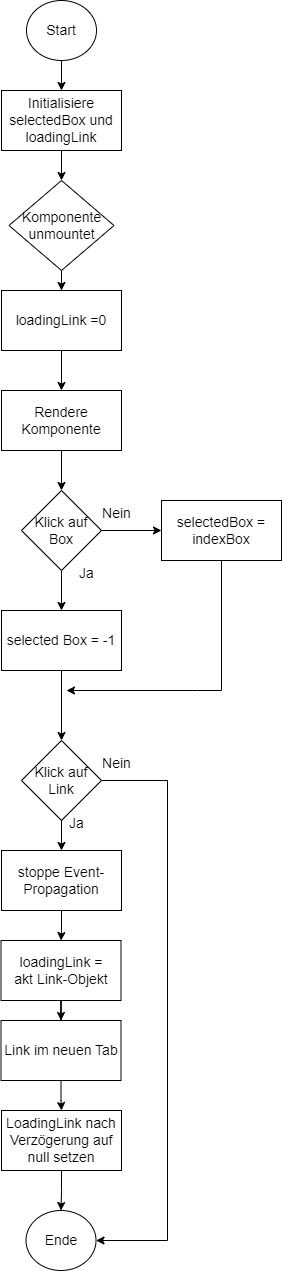
\includegraphics[height=0.7\textheight]{images/PAPLinks}}
	\caption{PAP Links}
\end{figure}
\begin{figure}[htbp]
	\centering
	\fbox{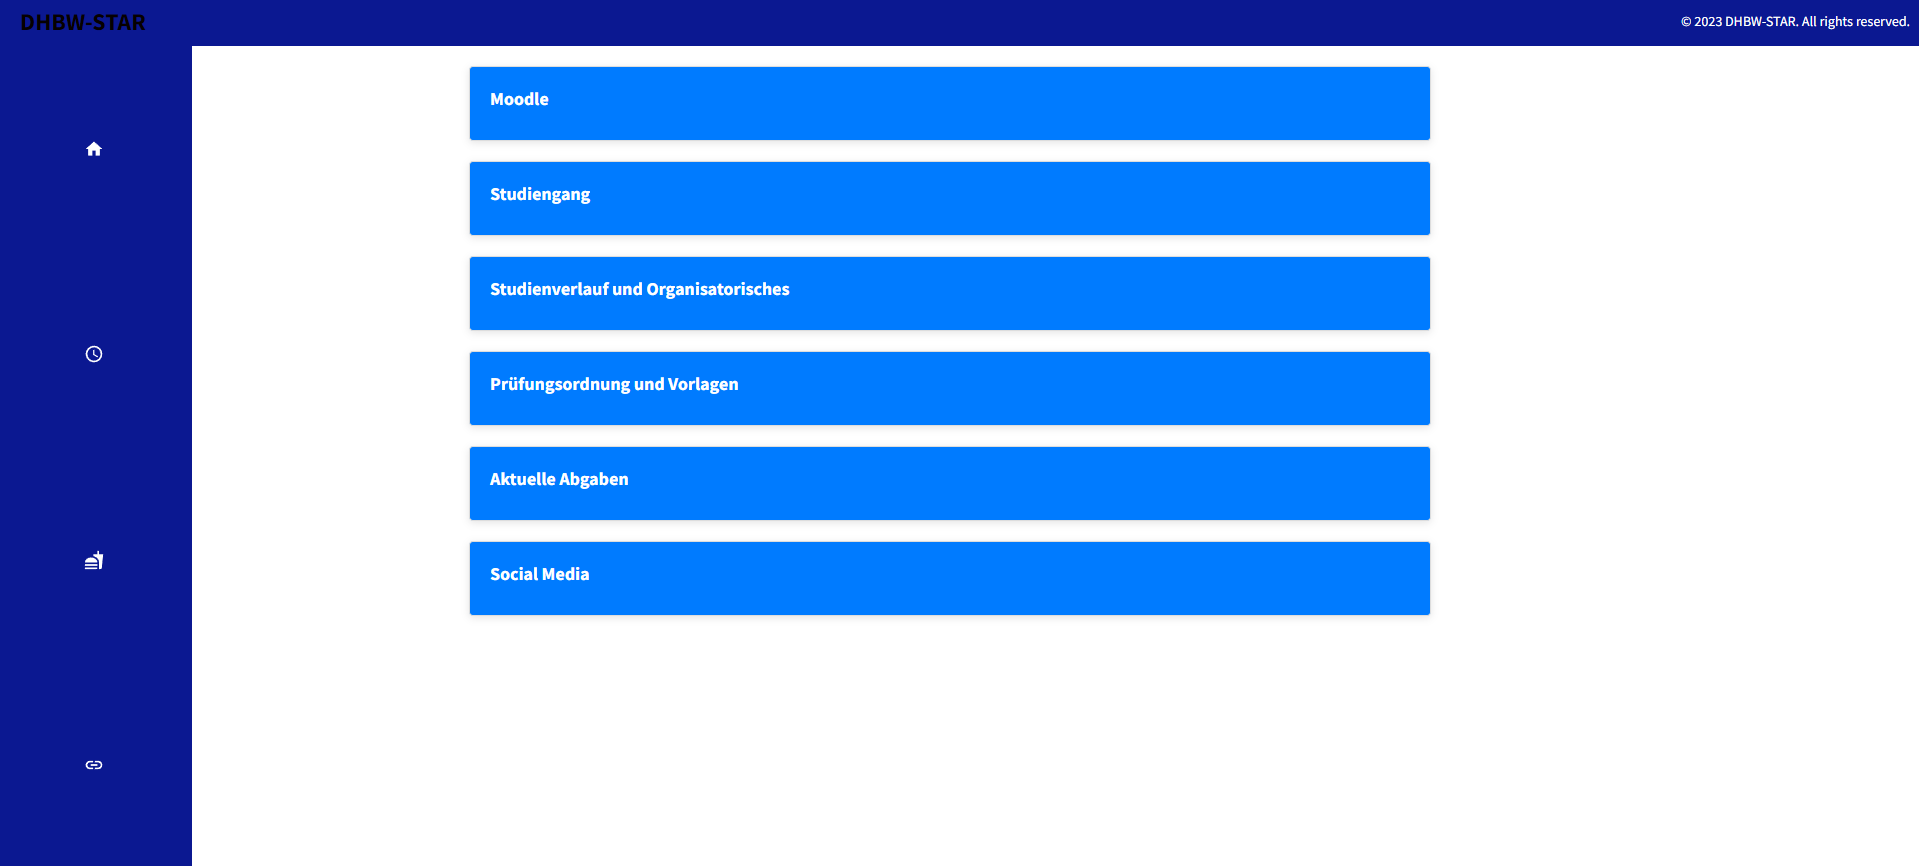
\includegraphics[height=0.3\textheight]{images/Links}}
	\caption{Links-Website}
\end{figure}
\newpage
\subsubsection{Implementierung}
Die Komponente \emph{Links} definiert zunächst eine Array-Struktur \emph{links}, die die verschiedenen Kategorien von Links und die jeweiligen Linkobjekte selbst enthält. Jedes Linkobjekt besteht aus einem Titel und einer URL.  
Der \emph{useState}-Hook wird verwendet, um zwei interne Zustandsvariablen zu definieren. \emph{selectedBox} verfolgt, welches Linkfeld gerade ausgewählt ist, und \emph{loadingLink} verfolgt, welcher Link gerade geladen wird.\\  
Der \emph{useEffect}-Hook wird verwendet, um den Status \emph{loadingLink} zurückzusetzen, wenn die Komponente nicht zusammengebaut ist. Hierbei handelt es sich um eine Sicherheitsmaßnahme, um sicherzustellen, dass der Status korrekt zurückgesetzt wird und es nicht zu unerwarteten Statusänderungen kommt, wenn Komponenten in  Zukunft wieder zusammengebaut werden. Die Funktion \emph{handleBoxClick} wird verwendet, um den Status der \emph{selectedBox} zu aktualisieren, wenn auf die Box geklickt wird. Durch erneutes Auswählen eines bereits ausgewählten Felds wird dessen Auswahl aufgehoben (d. h. \emph{selectedBox} wird auf -1 gesetzt). \\
Die Funktion \emph{handleLinkClick} dient zur Steuerung des Link-Klickverhaltens. Dadurch wird verhindert, dass das Standardereignisverhalten den Status \emph{loadingLink} aktualisiert und den Link in einem neuen Tab öffnet. Anschließend wird nach einer Verzögerung von 2000 ms der Status \emph{loadingLink} zurückgesetzt.  Die Rendermethode der Komponente durchläuft das Array \emph{links} und erstellt ein Element für jedes Feld und die darin enthaltenen Links. CSS-Klassen für  Boxen und Links werden basierend auf ihrem aktuellen Status dynamisch generiert.\\
Dies ist der zusammenhängende Code der Link-Komponente:
\begin{lstlisting}[language=JavaScript,
	frame=single,           % Ein Rahmen um den Code
	framexleftmargin=15pt,  % Rahmen link von den Zahlen
	style=algoBericht,
	label={Links-Komponente},
	captionpos=b ,          % Caption unter den Code setzen
	caption={Links-Komponente}]
import React, { useState,useEffect } from "react";
import "./Link.css";
const Link = () => {
  const links = [
  {
  	\\ Ein Haufen Links die fuers Studieren wichtig sind.
  	\\........................................
  }
];

  useEffect(() => {
    return () => {
      setLoadingLink(null); // Setzt den Ladezustand zurueck, 
      wenn die Komponente unmountet wird
  };}, []);
  const [selectedBox, setSelectedBox] = useState(-1);
  const [loadingLink, setLoadingLink] = useState(null); 
  // Initialer State zu null
  const handleBoxClick = (index) => {
    if (selectedBox === index) {
      setSelectedBox(-1);} 
    else {
    	setSelectedBox(index);
    }};
  const handleLinkClick = (e, boxIndex, linkIndex, link) => {
  	e.stopPropagation();
  	setLoadingLink({ boxIndex, linkIndex }); 
  	// Setzen Sie den Lade-Link auf das aktuelle Link-Objekt
  	window.open(link.url, "_blank");
	
    setTimeout(() => {
      setLoadingLink(null); // Setzt den Lade-Link 
      nach einer Verzoegerung zurueck
  }, 2000);};

 return (
 <div className="link-collection">
 {links.map((box, boxIndex) => (
 	<div key={boxIndex}
 	className={`link-box ${selectedBox === boxIndex ? 
 			"expanded" : ""}`}
 	onClick={() => handleBoxClick(boxIndex)}>
      <h3>{box.title}</h3>+
      <ul>
        {box.items.map((link, linkIndex) => (
         <li key={linkIndex}>
         <a className={loadingLink && 
         	loadingLink.boxIndex === boxIndex && 
         	loadingLink.linkIndex === linkIndex 
         	? "loading" : ""}
          onClick={(e) => handleLinkClick(
          	e, boxIndex, linkIndex, link)}>
          {link.title}
          </a>
          </li>))}
       </ul>
       </div>
		))}
	</div>
	);
};
export default Link;

\end{lstlisting}

Die Implementierung dieser Komponente ermöglicht eine bequeme und effiziente Darstellung von Linkgruppen. Die Struktur und das Verhalten der Komponenten sind klar und intuitiv, und der Einsatz von Statusverwaltung und Event-Handlern stellt sicher, dass die Komponenten korrekt auf Benutzerinteraktionen reagieren und  aktualisiert werden. Durch die Verwendung von React für diese Komponente ist sie wiederverwendbar und lässt sich leicht in andere Teile einer größeren Anwendung integrieren.
\newpage
\section{Zusammenfassung}
DHBW-Star ist ein  neues Webportal-Angebot für Studierende der DHBW Karlsruhe. Es wurde  entwickelt, um einen zentralen, benutzerfreundlichen Zugangspunkt zu allen relevanten Ressourcen und Informationen bereitzustellen. Das Portal vereint die drei Hauptkomponenten Stundenplan, Essensplan und Linksammlung und ist auf die spezifischen Bedürfnisse der Studierenden zugeschnitten. 
Um sicherzustellen, dass DHBW-Star den tatsächlichen Bedürfnissen der Studierenden entspricht und einen echten Mehrwert bietet, haben wir eine Umfrage durchgeführt, um Feedback und Verbesserungsvorschläge zu sammeln.
Diese Umfrage wird in den nächsten zwei Kapiteln erklärt und ausgewertet.
\newpage
\section{Docker}

Damit die React App vom System unabhängig funktioniert, läuft sie in einem Docker Container. Dadurch werden Probleme mit unterschiedlichen Programmversionen und Konfigurationen verhindert.
Da die geplante Mensa API nicht funktioniert, wird als Alternative ein Container verwendet, der die Mensa API lokal bereitstellt.

\subsection{Die Dockerfile, compose.yaml und .env Dateien}

Für den React Containers wird ein Dockerfile Datei benötigt. In dieser wird beschrieben wie der Container zusammengebaut wird. Ein neuer Container kann auf vorhanden aufbauen oder komplett neu erstellt werden.

\begin{lstlisting}[language=vhdl,
	frame=single,           % Ein Rahmen um den Code
	framexleftmargin=15pt,  % Rahmen link von den Zahlen
	style=algoBericht,
	label={Dockerfile},
	captionpos=b           % Caption unter den Code setzen
	caption={Dockerfile für DHBW-Star}]
FROM node:current-alpine

RUN mkdir /reactApp
WORKDIR /reactApp

# Install React and dependencies
COPY . .
RUN npm init -y
RUN npm install express cors axios
RUN npm install
RUN npm install ical.js
RUN npm install -D concurrently
RUN yarn build

# Start both React app and proxy server
CMD ["npm", "run", "start:all"]
\end{lstlisting}

Für DHBD Star wird der node Container von Dockerhub.com als Basis verwendet. Dieser besteht aus \emph{alpine}, einem minimalistischen Betriebssystem und NoteJS welcher für React benötigt wird.
Mit \emph{COPY} werden die Dateien des Projekts in den Container kopiert und mit \emph{RUN npm init} und \emph{RUN npm install} werden die benötigten Pakete für NoteJS installiert.
Zum Schluss wird mit \emph{RUN yarn build} das React Projekt gebaut und mit \emph{CMD ["npm", "run", "start:all"]} React und der Proxy gestartet. Der \emph{CMD} befehlt wird beim erstellen eines Container aus dem Image, immer ausgeführt. 

Damit die Mensa API und React zusammen starten, wird die \emph{compose.yaml} Datei und Docker compose verwendet.

\begin{lstlisting}[language=vhdl,
	frame=single,           % Ein Rahmen um den Code
	framexleftmargin=15pt,  % Rahmen link von den Zahlen
	style=algoBericht,
	label={Dockerfile},
	captionpos=b           % Caption unter den Code setzen
	caption={compose.yaml für DHBW-Star}]
version: '3.9'
services:
  react-app:
    build:
      dockerfile: ./Dockerfile
    tags:
      - "react:latest"
    ports:
      - "3003:3003"
      - "3002:3002"
    volumes:
      - ./src:/reactApp/src:ro
      - ./proxy-server.js:/reactApp/proxy-server.js:ro
      - ./.env:/reactApp/.env:ro
  mensa-api:
    image: meyfa/ka-mensa-api
    ports:
      - "3001:8080"
    environment:
      - MENSA_CORS_ALLOWORIGIN=*
\end{lstlisting}

Für den Service \emph{react-app} (DHBW Star) wird mit \emph{build} die oben beschrieben Dockerfiel Datei angeben. Somit baut der Befehl \emph{docker compose --build} ein neue Image mit dem React Projekt.
Der \emph{tags} gibt dem Container einen eindeutigen Namen.
Mit \emph{ports} werden die Ports vom Proxy(3002) und React (3003) nach außen frei gegeben.
Damit bei kleineren Änderungen im Projekt nicht immer ein neues Image erstellt werden muss, wird mit \emph{volums} die Projektdateien in den laufenden Container eingebunden.
Für die \emph{mensa-api} wird noch die Umgebungsvariable \emph{MENSA\_CORS\_ALLOWORIGIN=*} definiert.

Um die Container an unterschiedliche Gegebenheiten des Systems anpassen zu können, ohne etwas am React Projekt ändern zu müssen, bietet docer compose die Möglichkeit Umgebungsvariablen aus einer \emph{.env} Datei heraus zu definieren.
Da diese nicht teil von git sein sollte, wird eine \emph{.env\_template} angelegt. In dies stehen sind die verwendeten Umgebungsvariable mit Beispielen drin.
React verlangt für alle Umgebungsvariablen, die in der App zur Verfügung stehen sollen, dass sie mit \emph{REACT\_APP\_} beginnen.

\begin{lstlisting}[language=vhdl,
	frame=single,           % Ein Rahmen um den Code
	framexleftmargin=15pt,  % Rahmen link von den Zahlen
	style=algoBericht,
	label={Dockerfile},
	captionpos=b           % Caption unter den Code setzen
	caption={.env für DHBW-Star}]
REACT_APP_MENSA_ADDRESS=http://localhost:3001 
REACT_APP_PROXY_ADDRESS=http://localhost:3002
PROXY_PORT=3002
PORT=3003
\end{lstlisting}

\emph{REACT\_APP\_MENSA\_ADDRESS} und \emph{REACT\_APP\_PROXY\_ADDRESS} sind die Adressen der Services. Dies müssen mit der in \emph{compose.yaml} definierten Ports übereinstimmen. 

\section{Webserver}
Damit das Projekt auch über das Internet erreichbar ist, wird ein Root-Webserver mit einer Domain Adresse verwendet. Auf diesem ist bereits Docker, Nginx und Certbot Installiert.
Per github.com wird das Projekt auf den Server kopiert und die \emph{.env} Datei angepasst. Die Ports bleiben die Selben, nur das \emph{localhost} wird durch die Subdomains \emph{mensa.Domain} für den Mensa Container und \emph{ical.Domain} für den Proxy ersetzt.

Damit die Container unter ihrer Subdomain erreichbar sind, müssen diese in der Nginx Konfiguriert werden. In der Datei \emph{.../sites-enabled/star.conf} wird für jeden Service mit \emph{proxy\_pass} eine Weiterleitung eingerichtet.
Da auf dem Server bereits andere Webdienst laufen, ist Startseite unter der Subdomain \emph{star.Domain} erreichbar. Mit \emph{Certbot} werden noch SSL Zertifikate für alle Subdomains erstellt und automatisch eingerichtet.

Nach dem Neustart von Nginx, steht DHBW Star für alle Tester zur Verfügung.

